% !TEX root = main.tex

\section{知识表示与推理}
% First-order logic: syntax and semantics
% Soundness and completeness of proof procedures
% Converting first-order formulas into clausal form
% Unification and MGU
% Resolution proof: forward chaining and refutation
% Answer extraction

\subsection{基本概念}
一阶逻辑(First-Order Logic,FOL)
\begin{itemize}
	\item 个体/常量(0-arity)
	\item 一元(unary)谓词:$A(x),B(x)$
	\item 关系/二元谓词:$L(x,y)$
\end{itemize}

\begin{definition}[项(term)]
每一个变量都是一个项。
若$t_1,\ldots,t_n$都为项,且$f$为$n$参数的的函数符号,则$f(t_1,\ldots,t_n)$是一个项。
\end{definition}
\begin{definition}[公式(formular)]
公式包括以下几种情况:
\begin{itemize}
\item 若$t_1,\ldots,t_n$都是项,且$P$是$n$元的谓词符号,则$P(t_1,\ldots,t_n)$是一个公式
\item 若$t_1,t_2$都是项,那么$(t_1=t_2)$是一个原子公式
\item 若$\alpha,\beta$都是公式,$v$是一个变量,则$\lnot\alpha,(\alpha\land\beta),(\alpha\lnot\beta),\exists v.\alpha,\forall v.\alpha$都是公式
\end{itemize}
注意公式中的变量是自由的(free)还是约束的(bound),通过全称特称符号可进行约束。
没有自由变量的公式称为句子(sentence)。
\end{definition}
\begin{definition}[替换]
$\alpha[v/t]$表示$\alpha$中所有自由出现的$v$都用项$t$替代
\end{definition}
\begin{definition}[解释(interpretation)]
一个解释是一个对(pair)$\mI=\lrang{D,I}$,其中
\begin{itemize}
	\item $D$是论域,可以是任何非空集
	\item $I$是从谓词到函数符号的映射
	\item 若$P$是一个$n$元谓词符号,则$I(P)$是一个在$D$上的$n$元关系,即$I(P)\subset D^n$。
	如$p$是一个常量/命题符号,则$I(p)\in\{True,False\}$。
	\item 若$f$是一个$n$元函数符号,则$I(f)$是一个在$D$上的$n$元函数,即$I(f):D^n\to D$。
	如$c$是一个零元常量符号,则$I(c)\in D$。
\end{itemize}
\end{definition}
\begin{definition}[赋值(denotation)]
变量指派(assignment)$\mu$是一个从变量集合到论域$D$的映射
\[\begin{aligned}
\norm{v}_{\mI,\mu}&=\mu(v)\\
\norm{f(t_1,\ldots,t_n)}_{\mI,\mu}&=I(f)(\norm{t_1}_{\mI,\mu},\ldots,\norm{t_n}_{\mI,\mu})
\end{aligned}\]
\end{definition}
\begin{definition}[满足]
$\mI,\mu\models\alpha$读作$\mI,\mu$满足$\alpha$
\begin{itemize}
	\item $\mI,\mu\models P(t_1,\ldots,t_n)\iff\lrang{\norm{t_1}_{\mI,\mu},\ldots,\norm{t_n}_{\mI,\mu}}\in I(P)$
	\item $\mI,\mu\models(t_1=t_2)\iff\norm{t_1}_{\mI,\mu}=\norm{t_2}_{\mI,\mu}$
\end{itemize}
同样也有命题逻辑的一些性质
\begin{itemize}
	\item $\mI,\mu\models\lnot\alpha\iff\mI,\mu\not\models\alpha$
	\item $\mI,\mu\models(\alpha\land\beta)\iff(\mI,\mu\models\alpha\land\mI,\mu\models\beta)$
	\item $\mI,\mu\models(\alpha\lor\beta)\iff(\mI,\mu\models\alpha\lor\mI,\mu\models\beta)$
	\item $\mI,\mu\models\exists v.\alpha\iff(\exists d\in D:\mI,\mu\{d;v\}\models\alpha)$
	\item $\mI,\mu\models\forall v.\alpha\iff(\forall d\in D:\mI,\mu\{d;v\}\models\alpha)$
\end{itemize}

令$S$为句子的集合,若对于所有$\alpha\in\mI,\mI\models\alpha$,则称$\mI$满足$S$,记作$\mI\models S$,$\mI$又被称为$S$的一个模型。
若$S$是可满足的,则存在$\mI$使得$\mI\models S$。
\end{definition}
\begin{example}
通常的问题是下列句子集合是否是可满足的
\[\{\forall x(P(x)\to Q(x)),P(a),\lnot Q(a)\}\]
即是否存在这样的解释/变量赋值使全部句子都成立。
\end{example}

\begin{definition}[蕴含(entail)]
$S\models\alpha$是指对于任意满足$\mI\models S$的$\mI$有$\mI\models\alpha$,读作$S$蕴含$\alpha$或$\alpha$是$S$一个逻辑结果(consequence)。
注意$\{\alpha_1,\ldots,\alpha_n\}\models\alpha$当且仅当$\alpha_1\land\cdots\land\alpha_n\to\alpha$合法,当且仅当$\alpha_1\land\cdots\land\lnot\alpha$不可满足。
\end{definition}
\begin{example}
令知识库$KB$为句子集合,$\alpha$为一个询问,想要知道知识库是否能推出询问,即求蕴含$KB\models\alpha$。
若要证明$KB\not\models\alpha$,则只需给出一个解释满足$KB$但不满足$\alpha$。
\end{example}

\subsection{推理}
\subsubsection{归结}
\begin{definition}[子句(clause)]
文字(literal)是原子公式或它的取反,一个子句是文字的析取(disjunction),如$p\lor\lnot r\lor s$,写作$(p,\lnot r,s)$。
特殊地,空子句$()$代表为假。
公式(formula)则是子句的合取(conjunction)。
\end{definition}

\begin{definition}[归结(resolution)]
从两条子句$\{p\}\cup c_1$和$\{\lnot p\}\cup c_2$中推出子句$c_1\cup c_2$的过程称为归结。
\end{definition}
\begin{definition}[获取(derivation)]
句子序列$c_1,\ldots,c_n=c$,对于每一个$c_i$,或者$c_i\in S$,或者$c_i$是先前\textemph{两个子句}的归结,这个过程称为获取,记为$S\vdash c$。
\end{definition}
\begin{theorem}
若$S\vdash c$,则$S\models c$
\end{theorem}
但注意其逆命题并不成立,考虑$(p)\models(p,q)$,但是$(p)\nvDash(p,q)$。

\begin{theorem}
$S\vdash()\iff S\models()\iff S$是不可满足的
\end{theorem}

进而得到基于归结的推理过程:反驳(refutation),即$KB\models\alpha\iff KB\land\alpha$是不可满足的
\begin{itemize}
	\item 将$KB$和$\lnot\alpha$改写为子句形式构成$S$
	\item 检测是否$S\vdash()$
\end{itemize}
\begin{figure}[H]
\centering
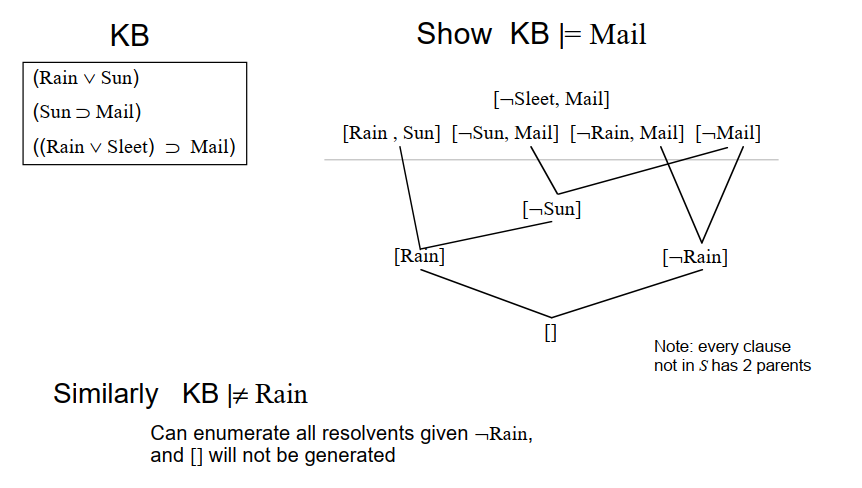
\includegraphics[width=0.8\linewidth]{fig/refutation.png}
\end{figure}

利用归结(两条文字合一变真删除)看是否能得到空子句。

\subsubsection{子句形式转换}
\begin{itemize}
	\item 消除蕴含:$A\to B\iff \lnot A\lor B$
	\item 否定内移:德摩根定律
	\item 标准化变量:重命名变量使得每一个量词都是唯一的
	\item 消除存在量词(skloemize):引入新的函数符号,如$\forall x P(x)$改为$P(g(y))$
	\item 改为前缀形式:只有全局量词,且名字均不同
	\item 析取分配到合取
	\item 压平嵌套合取和析取
	\item 转化为子句:将量词全部移除,然后分离成几条子句
\end{itemize}
\begin{example} % T02-3
用归结判断下列句子是否可满足
\[(\exists x\forall y P(x,y)\lor\exists x\forall y Q(x,y))\to
\exists x\forall y(P(x,y)\lor Q(x,y))\]
\end{example}
\begin{analysis}
	按照子句形式的转换顺序,有
    \begin{itemize}
        \item 改写为归结的等价形式(消除蕴含)
        \[(\exists x\forall y P(x,y)\lor\exists x\forall y Q(x,y))\land\lnot
        (\exists x\forall y(P(x,y)\lor Q(x,y)))\]
        \item 否定内移
        \[(\exists x\forall y P(x,y)\lor\exists x\forall y Q(x,y))\land
        (\forall x\exists y (\lnot P(x,y)\land \lnot Q(x,y)))\]
        \item 标准化变量
        \[(\exists x\forall y P(x,y)\lor\exists z\forall w Q(z,w))\land
        (\forall a\exists b (\lnot P(a,b)\land \lnot Q(a,b)))\]
        \item Skolemize
        \[(\forall y P(x,y)\lor \forall w Q(z,w))\land
        (\forall a (\lnot P(a,f(a))\land \lnot Q(a,f(a))))\]
        \item 改为前缀形式
        \[\forall y\forall w\forall a ((P(x,y)\lor Q(z,w))\land
        (\lnot P(a,f(a))\land \lnot Q(a,f(a))))\]
        \item 变成子句形式
        \begin{itemize}
            \item [1.] $P(x,y),Q(z,w)$
            \item [2.] $\lnot P(a,f(a))$
            \item [3.] $\lnot Q(a,f(a))$
        \end{itemize}
    \end{itemize}
    归结过程如下
    \begin{enumerate}
        \item [4.] $R[1a,2]\{a=x,y=f(a)\}$:$(Q(z,w))$
        \item [5.] $R[3,4]\{a=z,w=f(a)\}$:$()$
    \end{enumerate}
    总结即当$a=x,y=f(a),a=z,w=f(a)$时得到归结结果,题目中的式子成立。
    \textemph{(注意变量写左边,常量写右边)}
\end{analysis}

\subsubsection{合一}
归结过程中可能需要合一(unification),用来消除两个子句中不同的变量。
\begin{definition}[合一子(unifier)]
令公式$f$和$g$语义等价的替换$\sigma$称为$f$和$g$的合一子
\end{definition}
\begin{example}
$P(f(x),a)$和$P(y,f(w))$不能被合一,因没有令$a=f(w)$的替换使得两者相同
\end{example}

\begin{definition}[最一般合一子(Most General Unifier, MGU)]
两个公式$f$和$g$的替换$\sigma$是MGU,若
\begin{itemize}
	\item $\sigma$是一个合一子
	\item 对于其他合一子$\theta$必然存在第三个替换$\lambda$使得$\theta=\sigma\lambda$
\end{itemize}
也就是说其他的合一子都比$\sigma$更特殊(specialized)。
\end{definition}
\begin{example}
考虑$P(f(x),z)$和$P(y,a)$
\begin{itemize}
	\item $\sigma=\{y=f(a),x=a,z=a\}$是一个合一子,但不是MGU
	\item $\theta=\{y=f(x),z=a\}$是一个MGU
	\item $\sigma=\theta\lambda$,其中$\lambda=\{x=a\}$
\end{itemize}
\end{example}

计算MGU的算法:不断代入新的元,使其一致
\begin{figure}[H]
\centering
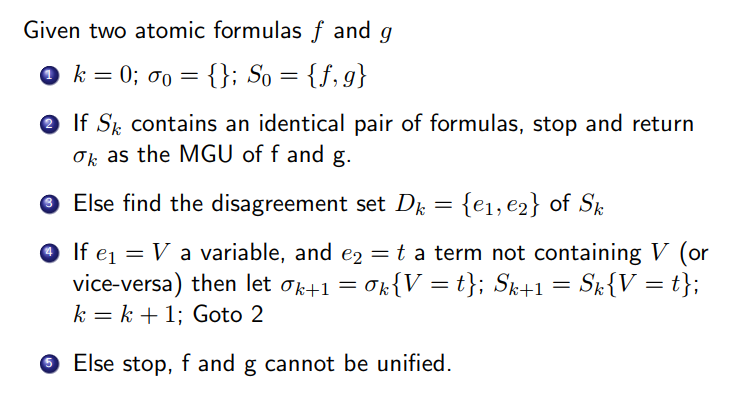
\includegraphics[width=0.8\linewidth]{fig/MGU.png}
\end{figure}

\subsubsection{完整例子}

\paragraph{基于反驳的归结推理}
\begin{example}
下面是一个例子
\begin{figure}[H]
\centering
\begin{tabular}{c}
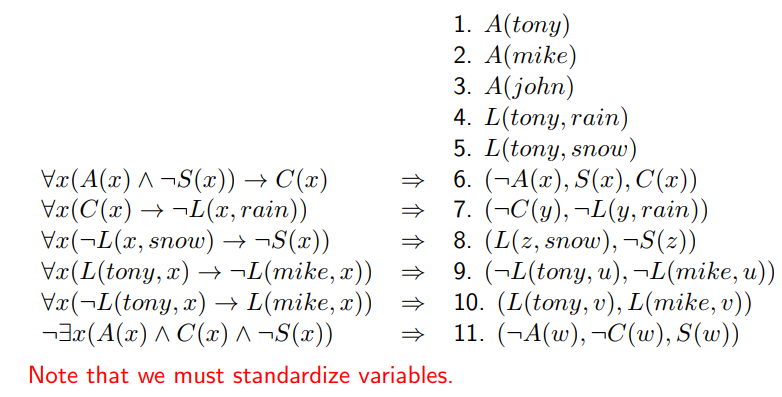
\includegraphics[width=0.8\linewidth]{fig/alpine_club_eg1.png}\\
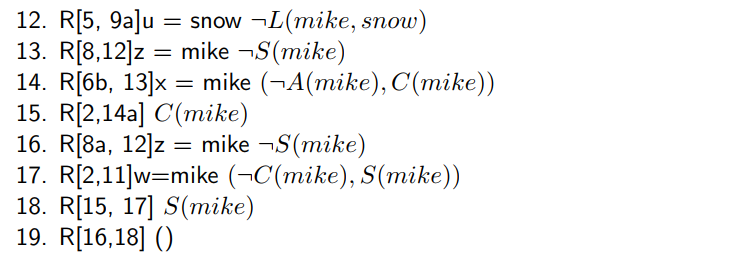
\includegraphics[width=0.8\linewidth]{fig/alpine_club_eg2.png}
\end{tabular}
\end{figure}
\end{example}

\paragraph{答案抽取(answer extraction)}
\begin{itemize}
\item 将询问$\exists xP(x)$用$\exists x[P(x)\land\lnot\text{answer}(x)]$替换
(因为取非后变成$\forall x P(x)\implies \text{answer}(x)$)
\item 直到获得任意子句只包含答案的谓词
\end{itemize}
\begin{example}
对下列查询进行归结及答案查询
\begin{itemize}
	\item Whoever can read $R(x)$ is literate $L(x)$
	\item Dolphins $D(x)$ are not literate
	\item Flipper is an intelligent dolphin $I(x)$
\end{itemize}
Who is intelligent but cannot read?
\end{example}
\begin{analysis}
对语句进行形式化
\begin{center}
\begin{tabular}{lll}
$\forall x (R(x)\to L(x))$ & 1 & $(\lnot R(u),L(u))$\\
$\forall x (D(x)\to \lnot L(x))$ & 2 & $(\lnot D(v),\lnot L(v))$\\
$D(Flip)\land I(Flip)$ & 3 & $D(Flip)$\\
 & 4 & $I(Flip)$\\
Q:$\exists x (I(x)\land\lnot R(x))$ & 5 & $(\lnot I(y),R(y),answer(y))$\\\hline 
$R[4,5]/y=Flip$ & 6 & $(R(Flip),answer(Flip))$\\
$R[1,6]/u=Flip$ & 7 & $(L(Flip),answer(Flip))$\\
$R[2,7]/v=Flip$ & 8 & $(\lnot D(Flip),answer(Flip))$\\
$R[3,8]$ & 9 & $(answer(Flip))$
\end{tabular}
\end{center}
因此得到Flipper是聪明的但是不能阅读
\end{analysis}